\documentclass[a4paper,11pt]{article}
\usepackage{jinstpub}

%%--- Packages ---------------------------------------------------------------
\usepackage{amsmath}
\usepackage{amssymb}
\usepackage{graphicx}
\usepackage{booktabs}
\usepackage{array}
\usepackage{float}
\usepackage{xspace}
\usepackage{microtype}

\graphicspath{{figures/}{figures/inclusive_fit/}{figures/stratified_tests/}}

%%--- Convenience macros -----------------------------------------------------
\newcommand{\MET}{\ensuremath{E_{\mathrm{T}}^{\mathrm{miss}}}\xspace}
\newcommand{\pTZ}{\ensuremath{p_{\mathrm{T}}(Z)}\xspace}
\newcommand{\chisq}{\ensuremath{\chi^2}\xspace}
\newcommand{\Dchisq}{\ensuremath{\Delta\chi^2}\xspace}
\newcommand{\zmumu}{\ensuremath{Z\!\to\!\mu^+\mu^-}\xspace}

%%--- Title and author -------------------------------------------------------
\title{Non-identifiability of Nuisance Mechanisms in Reduced Collider
  Observables: Evidence from CMS Open Data}

\author{Michael Blumhardt}
\affiliation{Independent Researcher}
\emailAdd{blumhardt@gmail.com}

%%--- Abstract (single paragraph, JINST style) -------------------------------
\abstract{%
Inclusive goodness-of-fit validation of reduced collider observables can
admit multiple nuisance explanations when high-dimensional event records are
compressed into summary statistics.
This study investigates this identifiability limitation using the missing
transverse momentum distribution in \zmumu events reconstructed from CMS
Open Data (233\,524 selected events from the DoubleMuon 2016 dataset).
A recoil-response distortion (Family~A) is injected at a known working point
and used as the validation target.
A topology-mixture reweighting (Family~B), operating through an incompatible
mechanism, reproduces the inclusive distribution with
$\chi^2/\mathrm{dof} = 3.13/11$ ($p = 0.989$), demonstrating practical
non-identifiability in the inclusive projection despite the large event
sample.
A physically motivated perturbation derived from CMS unclustered-energy
systematic-variation branches (Family~C) lies near the boundary of inclusive
discriminability ($\chi^2 = 18.28$, $p = 0.075$).
Conditional projections stratified by \pTZ and jet multiplicity recover
discrimination without refitting: the recoil-stratified test yields
$\Delta\chi^2 = 1432$ in the highest-recoil bin, while the jet-multiplicity
test yields $\Delta\chi^2 = 3415$ in the ${\geq}2$-jet category.
These results show that compression of collider events into reduced
observable representations can induce nuisance degeneracies invisible to
inclusive validation but detectable through simple conditional diagnostics.}

\keywords{Analysis and statistical methods,
  Performance of High Energy Physics Detectors,
  Detector modelling and simulations}

%%===========================================================================
\begin{document}
\maketitle
\flushbottom

%%===========================================================================
\section{Introduction}
\label{sec:intro}
%%===========================================================================

Analyses performed on compressed or reduced-tier datasets face an intrinsic
statistical challenge: distinct physical mechanisms can produce
indistinguishable predictions for marginal observables when latent structure
is integrated out.
In such settings, agreement between model and data in a one-dimensional
validation distribution does not guarantee that the underlying nuisance
mechanism is uniquely identified.
This problem becomes particularly relevant for external analyses using
publicly released collider datasets, where the available observables are
intentionally compressed relative to the full detector reconstruction.

Collider analyses typically operate on reduced observables obtained from
high-dimensional event records.
Denoting the full reconstructed event record as $X$ and the reduced
observable as $Y = R(X)$, the projection $R$ discards information present
in $X$ that is not retained in $Y$.
Because $Y$ arises from such a projection, it is not generally a sufficient
statistic for the underlying nuisance mechanisms: distinct values of a
nuisance parameter $\theta$ can produce the same distribution $P(Y|\theta)$
even when $P(X|\theta)$ differs.
Consequently, distinct physical mechanisms can produce indistinguishable
inclusive distributions of a reduced observable even when their full-event
descriptions differ.

In the broader statistics literature this situation corresponds to an
identifiability problem, in which distinct latent mechanisms produce
indistinguishable predictions once high-dimensional structure is compressed
into low-dimensional summary observables.
Modern collider analyses normally mitigate such degeneracies using
simultaneous multi-bin profile likelihood fits across orthogonal control
regions, but these techniques rely on access to the full observable space and
collaboration-internal systematic variations that are not available in
reduced-tier public datasets.

Missing transverse momentum provides a particularly useful observable for
examining this issue.
\MET is a highly composite quantity, constructed from the vector sum of
reconstructed particle-flow candidates and subject to corrections that depend
on jet calibration, pileup mitigation, and detector response~\cite{CMS:JES2017}.
In the NanoAOD format used in CMS Open Data, \MET is exposed primarily as a
reconstructed end-product rather than as a quantity derived from constituent
detector information.
This makes \MET an ideal setting for studying how reduced observability
affects the identifiability of nuisance mechanisms.
This study does not evaluate the CMS reconstruction pipeline itself; rather,
it examines inference limits that arise when analyses operate on reduced
public data products such as NanoAOD.

In parallel, CMS has released a substantial fraction of its LHC data to the
public, enabling external researchers to perform analyses using well-defined
reduced data tiers such as NanoAOD.
These releases have supported a growing body of peer-reviewed work, including
studies of jet substructure, dimuon spectra, and methodological analyses
based on public data.
However, the reduced-tier formats provided for open data necessarily compress
detector-level information and expose high-level observables, such as \MET,
primarily as reconstructed end-products.
While this design greatly improves accessibility, it also limits the range of
detector and reconstruction effects that can be explicitly modelled or varied
by external analysts.

As a consequence, external analyses using CMS Open Data face a distinct
interpretive challenge: even when agreement between data and simulation is
observed for standard validation distributions, it is not always clear whether
the underlying causal mechanisms responsible for that agreement are uniquely
determined by the available observables.
In other words, agreement does not automatically imply identifiability.
This distinction is particularly relevant for \MET, where multiple
detector-related effects can plausibly contribute to similar distributional
features.

The possibility that distinct nuisance mechanisms can produce
indistinguishable predictions for marginal observables is well recognised in
collider statistics.
Contemporary LHC analyses typically address such degeneracies using
multidimensional control regions and simultaneous profile-likelihood fits
across correlated observables, often supplemented by auxiliary calibration
measurements~\cite{Cranmer:2014}.
More recently, simulation-based inference and related likelihood-learning
techniques have explored similar identifiability questions in
high-dimensional observable spaces~\cite{Valsecchi:2026,ATLAS:2024}.
These approaches implicitly rely on access to rich detector-level information
and extensive sets of systematic-variation branches available within
collaboration analysis frameworks.
By contrast, external analyses using CMS Open Data operate on compressed
representations such as NanoAOD, where many of the underlying degrees of
freedom are no longer directly accessible.
The present work therefore addresses a complementary question: to what extent
do competing nuisance explanations remain distinguishable when inference is
restricted to the reduced observable space available at the public data tier?

The present study addresses this issue by focusing on \zmumu events, which
provide a well-established standard candle for \MET studies.
In these events, genuine \MET is expected to be negligible, such that the
observed \MET distribution is dominated by instrumental effects.
The analysis is restricted to publicly available NanoAOD-level observables,
explicitly adopting the perspective of an external analyst operating within
the constraints of CMS Open Data.
Importantly, the degeneracy demonstrated here is constructed using real
collider events from CMS Open Data rather than purely simulated examples.
This allows the analysis to expose inference structure that arises in
practical collider datasets rather than in idealised Monte Carlo studies.

Rather than attempting to reproduce collaboration-grade \MET systematics or
to propose improvements to \MET reconstruction, the objective is to assess
the discriminating power of public-tier observables with respect to
competing, physically plausible nuisance explanations for \MET tails.
Two phenomenological nuisance families are examined, representing distinct
mechanisms by which the inclusive \MET distribution may be distorted: a
recoil-response scale distortion correlated with \pTZ, and a
topology-mixture reweighting that alters the relative population of
jet-multiplicity categories.
The two nuisance families correspond to perturbations arising at different
stages of the reconstruction pipeline, representing distinct physical
mechanisms rather than alternative parameterisations of a single model.

Using a controlled injection framework and a \chisq fit criterion, the
analysis evaluates whether these nuisance families can be tuned to reproduce
the same target \MET distribution and whether the inclusive projection is
sufficient to discriminate between them.
The effectiveness of stratified diagnostics --- conditioned on \pTZ and jet
multiplicity, both available in NanoAOD --- is further examined for their
ability to break the inclusive degeneracy.

The goal of this study is not to propose a new model of \MET, but to assess
whether competing nuisance explanations can be distinguished using only the
observables available in the NanoAOD data tier.

This work demonstrates that the inclusive missing transverse momentum
distribution in \zmumu events reconstructed from CMS Open Data admits
multiple nuisance explanations when analyses are restricted to the reduced
observable space available in NanoAOD.
In a controlled injection study, a topology-mixture reweighting model is
shown to reproduce the inclusive \MET distribution with
$\chi^2/\mathrm{dof} = 3.13/11$ ($p = 0.989$) despite operating through a
mechanism incompatible with the injected recoil distortion.
Conditional projections stratified by \pTZ and jet multiplicity restore
discrimination, yielding $\Delta\chi^2 = 1432$ and $\Delta\chi^2 = 3415$
in the most sensitive strata.
These results illustrate how compression of collider observables can induce
practical non-identifiability in inclusive validation tests and demonstrate
that simple stratified diagnostics provide an effective identifiability
check for analyses performed on reduced-tier public data.

Fig.~\ref{fig:identifiability_landscape} summarises the central argument of
this paper.
Distinct nuisance mechanisms can reproduce indistinguishable inclusive
distributions of a reduced observable, while conditional diagnostics reveal
statistically significant divergence.

\begin{figure}[t]
  \centering
  
\includegraphics[width=0.80\linewidth]{identifiability_landscape.pdf}
  \caption{Identifiability landscape illustrating compression-induced
    degeneracy in reduced collider observables.
    The horizontal axis shows inclusive fit quality ($\chi^2$) to the
    injected target \MET distribution; higher values indicate stronger
    inclusive agreement and deeper degeneracy risk.
    The vertical axis shows the maximum conditional discrepancy
    ($\Delta\chi^2$) across recoil and jet-multiplicity strata (symlog
    scale).
    Configurations in the upper-right region pass inclusive validation
    while producing large conditional discrepancies, illustrating how
    compression of collider events into reduced observables can mask
    mechanistic differences between nuisance models.
    Quantitative results are presented in Section~\ref{sec:results}.
    This visualisation summarises the central result of the analysis:
    inclusive goodness-of-fit alone does not guarantee mechanistic
    identifiability, whereas simple conditional projections restore
    discrimination even when the inclusive distribution appears
    statistically consistent.}
  \label{fig:identifiability_landscape}
\end{figure}

%%===========================================================================
\section{CMS Open Data and Analysis Scope}
\label{sec:data}
%%===========================================================================

The analysis presented in this work is based exclusively on publicly released
CMS Open Data corresponding to proton--proton collisions recorded in 2016 at
a centre-of-mass energy of 13\,TeV by the CMS detector.
The CMS Open Data programme provides external access to research-grade
datasets, associated Monte Carlo simulations, and documentation intended to
enable reproducible analyses outside the collaboration~\cite{CMSOpenDataGuide}.

\subsection{Open Data Tiers and Design Philosophy}

CMS Open Data are released in multiple data tiers that differ in information
content, file size, and intended use.
For Run~2 data, the NanoAOD format represents the most compact tier designed
for physics analysis, containing high-level reconstructed objects and derived
quantities in a flat ntuple structure~\cite{CMS:MiniNanoAOD,Rizzi:2019}.
NanoAOD is explicitly optimised for accessibility and computational
efficiency, enabling analyses to be performed without reliance on the full
CMS software stack or detector-level reconstruction code.

This design necessarily entails a loss of low-level information.
In particular, NanoAOD does not provide access to individual particle-flow
candidates, detailed reconstruction intermediates, or the full sequence of
corrections and calibrations applied internally within CMS.
As a result, certain detector effects --- especially those associated with
unclustered energy, rare reconstruction pathologies, or detailed pileup
mitigation algorithms --- cannot be independently recomputed or varied by
external analysts.

The present work explicitly embraces these constraints.
Rather than treating reduced observability as a limitation to be overcome,
such compression is treated as a defining feature of the inference problem
under study.

\subsection{\texorpdfstring{\MET}{MET} Representation in NanoAOD}

In NanoAOD, missing transverse momentum is provided as a reconstructed object
(\texttt{MET\_pt}, \texttt{MET\_phi}) that reflects the final CMS \MET
definition after standard corrections and pileup mitigation procedures~\cite{CMS:MET2019}.
While jet kinematics, muon kinematics, and basic pileup proxies (e.g.,
number of reconstructed primary vertices) are available, the internal
composition of \MET --- including contributions from unclustered energy ---
is not exposed.

Consequently, \MET in NanoAOD should be understood as an end-product
observable rather than a quantity that can be re-derived from constituent
objects.
This has important implications for causal interpretation: different
detector- or reconstruction-level mechanisms may map onto similar \MET
distributions without being distinguishable at the public tier.

The analysis in this work does not attempt to reverse-engineer or
reinterpret the CMS \MET reconstruction.
Instead, \MET is treated as an observable whose distributional behaviour is
to be compared between data and simulation under phenomenological
perturbations applied at the level of available observables.

\subsection{Scope of Simulation Use}

Monte Carlo simulation samples corresponding to $Z$+jets processes are used
as a reference model for comparison with data.
Consistent with the public-data context, only the simulation products
provided through the CMS Open Data portal are used, without access to
internal systematic variations or detector recalibration tools.

Nuisance models introduced in this work are therefore applied at the level
of the simulated \MET observable or via correlations with other available
high-level quantities.
These models are not intended to reproduce CMS systematic uncertainty
procedures, but to represent distinct, physically plausible explanations
that an external analyst could reasonably entertain given the accessible
information.

\subsection{Deliberate Scope Limitations}

For clarity, the following scope restrictions apply:
\begin{itemize}
  \item This work does not attempt to validate or supersede CMS \MET
    performance studies.
  \item No detector-level recalibration or re-reconstruction is performed.
  \item No claims are made regarding optimal \MET modelling or correction
    strategies.
  \item All conclusions are conditional on the information available at the
    NanoAOD tier.
\end{itemize}
Within this deliberately constrained scope, the analysis addresses a
narrower but well-defined question: to what extent can distinct instrumental
explanations for \MET tails be discriminated using public-tier observables
alone?

%%===========================================================================
\section{Event Selection}
\label{sec:selection}
%%===========================================================================

\subsection{Input Observables}

The selection and baseline analysis read the following NanoAOD branches from
the \texttt{Events} tree:
\begin{itemize}
  \item \textbf{Muon kinematics and identity:} \texttt{Muon\_pt},
    \texttt{Muon\_eta}, \texttt{Muon\_phi}, \texttt{Muon\_mass},
    \texttt{Muon\_charge}.
  \item \textbf{Muon quality:} \texttt{Muon\_tightId} (boolean),
    \texttt{Muon\_pfRelIso04\_all} (PF relative isolation,
    cone $\Delta R = 0.4$).
  \item \textbf{Missing transverse momentum:} \texttt{MET\_pt}.
  \item \textbf{Jets:} \texttt{Jet\_pt}, \texttt{Jet\_eta},
    \texttt{Jet\_phi}.
  \item \textbf{Event count:} \texttt{nMuon}.
\end{itemize}
No lower-level detector quantities are used.
The analysis operates entirely at the NanoAOD reconstructed-object tier.

\subsection{Muon Selection and Dimuon Construction}

A muon is retained if it satisfies all of the following requirements
simultaneously:
\begin{itemize}
  \item $p_{\mathrm{T}} > 15\,\mathrm{GeV}$
  \item $|\eta| < 2.4$
  \item \texttt{Muon\_tightId} $= 1$ (CMS Tight muon identification~\cite{CMS:Muon2018})
  \item \texttt{Muon\_pfRelIso04\_all} $< 0.15$ (PF relative isolation,
    $\Delta R = 0.4$ cone)
\end{itemize}
In addition, the leading muon in the selected pair must satisfy
$p_{\mathrm{T}} \geq 25\,\mathrm{GeV}$.

Dimuon pairs are formed by taking all unique two-muon combinations within
each event and retaining only opposite-sign pairs.
The invariant mass of each opposite-sign pair is computed from the
four-vector sum.
If multiple opposite-sign pairs satisfy the baseline selection, the $Z$
candidate is defined as the pair whose invariant mass is closest to the
nominal $Z$ boson mass ($91.1876\,\mathrm{GeV}$~\cite{PDG:2020}).

\subsection{$Z$-Candidate Definition}

A mass window requirement of $80\,\mathrm{GeV} \leq m(\mu^+\mu^-) \leq
100\,\mathrm{GeV}$ is applied as a hard selection cut.
The dimuon transverse momentum \pTZ is taken as the magnitude of the
transverse component of the four-vector sum of the two selected muons, and
serves as the primary recoil variable for the \pTZ stratification in
Section~\ref{sec:results}.

\subsection{Jet Cleaning and Jet-Multiplicity Definition}

A jet is included in the multiplicity count if it satisfies:
\begin{itemize}
  \item $p_{\mathrm{T}}(\text{jet}) > 30\,\mathrm{GeV}$
  \item $\Delta R(\text{jet},\,\mu_1) > 0.4$ \textbf{and}
    $\Delta R(\text{jet},\,\mu_2) > 0.4$
\end{itemize}
where $\Delta R = \sqrt{\Delta\eta^2 + \Delta\phi^2}$ and $\mu_1$,
$\mu_2$ are the two muons forming the selected $Z$ candidate.
Events are assigned to one of three exclusive jet-multiplicity categories:
0-jet, 1-jet, and $\geq\!2$-jet.
These three categories are used for the jet-multiplicity stratification in
Section~\ref{sec:results}.

\subsection{Analysis Sample}

The selection described above was applied to the full CMS Open Data
DoubleMuon 2016 NanoAOD dataset.
A total of 2\,147\,195 events were processed.
After applying all muon quality cuts, the opposite-sign requirement, the
leading muon $p_{\mathrm{T}}$ threshold of 25\,GeV, and the $Z$-mass window
of 80--100\,GeV, 233\,524 events were retained (overall selection efficiency
$\approx 10.9\%$).
This sample constitutes the analysis sample for all comparisons in
Section~\ref{sec:results}.

%%===========================================================================
\section{Nuisance Model Families}
\label{sec:models}
%%===========================================================================

\subsection{Motivation for Phenomenological Nuisance Families}

The nuisance models considered here are intentionally low-dimensional
phenomenological parameterisations.
Their purpose is not to reproduce collaboration-grade detector systematic
models, but to represent distinct classes of physical explanations for
distortions in the \MET distribution that an external analyst might
entertain when working with CMS Open Data.
Two families are considered, each parameterised by a single continuous
scalar.
Low dimensionality is deliberate: excessive model flexibility would trivially
explain any distributional feature, making non-identifiability uninformative.
The two families are mutually incompatible in mechanism: one alters the \MET
magnitude of individual events, the other alters the population weights
across event topologies.

\subsection{Fitting Strategy}

The identifiability test is implemented as a controlled injection.
Family~A is applied to the nominal \MET distribution at a known working
point $\alpha_0$, producing a target distribution.
Family~B is then independently fitted to the same target by grid search
over its parameter $\beta$.
Fit quality is quantified using the \chisq statistic:
\begin{equation}
  \chi^2 = \sum_k \frac{\bigl(h_k^{\mathrm{model}} -
    h_k^{\mathrm{target}}\bigr)^2}{h_k^{\mathrm{target}} + 1}
  \label{eq:chi2}
\end{equation}
where $h_k$ denotes the bin count in histogram bin $k$, and the
$(h_k^{\mathrm{target}}+1)$ denominator provides stability in bins with low
target occupancy.
Degrees of freedom for Family~B are $n_{\mathrm{bins}} - 1$.

\subsection{Family A --- Recoil-Response Distortion}

Family~A represents the hypothesis that \MET tails arise from a
miscalibrated hadronic recoil response.
The model modifies the event-level \MET as:
\begin{equation}
  \bigl(E_{\mathrm{T}}^{\mathrm{miss}}\bigr)'_i =
  \bigl(E_{\mathrm{T}}^{\mathrm{miss}}\bigr)_i \times
  \Bigl(1 + \alpha \cdot
    \frac{\mathrm{clip}\bigl(p_{\mathrm{T}}(Z)_i,\,0,\,100\bigr)}{100}
  \Bigr)
  \label{eq:familyA}
\end{equation}
where $\mathrm{clip}(\cdot,0,100)$ caps the effective recoil scale at
100\,GeV and $\alpha$ is the distortion amplitude.
The parameter search range is $\alpha \in [-0.30, +0.30]$ in steps of
$0.01$.
The injection working point used throughout this analysis is $\alpha_0 =
0.05$, corresponding to a 5\% maximum \MET scale distortion in the
highest-recoil events.
Family~A leaves the relative population of jet-multiplicity categories
unchanged.

\subsection{Family B --- Topology-Mixture Reweighting}

Family~B represents the hypothesis that \MET tails arise from a shift in
the event-topology composition of the sample rather than from a
miscalibration of the \MET scale within any given topology.
The model applies per-event weights according to jet multiplicity:
\begin{center}
\begin{tabular}{lc}
  \toprule
  Jet category & Weight \\
  \midrule
  0 jets   & $1$ \\
  1 jet    & $1 + \beta$ \\
  $\geq\!2$ jets & $1 + 2\beta$ \\
  \bottomrule
\end{tabular}
\end{center}
Weights are normalised so that the total weighted event count equals the
unweighted count.
The search range is $\beta \in [-0.40, +0.40]$ in steps of $0.01$.
Crucially, Family~B does not alter the \MET value of any individual event;
it changes only the effective population of each jet-multiplicity stratum.

\subsection{Mechanistic Contrast}

The two families modify the inclusive \MET distribution through
fundamentally different mechanisms:

\begin{table}[H]
  \centering
  \caption{Mechanistic contrast between nuisance families.}
  \label{tab:contrast}
  \begin{tabular}{lcc}
    \toprule
    & Family A & Family B \\
    \midrule
    Mechanism & Recoil-response distortion & Topology-mixture reweighting \\
    Parameter & $\alpha$ & $\beta$ \\
    Effect on event-level \MET & Scales \MET with \pTZ & None \\
    Effect on jet-category populations & None & Upweights multi-jet events \\
    Injection working point & $\alpha = 0.05$ & $\beta = +0.290$ (best fit) \\
    \bottomrule
  \end{tabular}
\end{table}

Family~A is sensitive to the recoil--\MET relationship and is exposed by
conditioning on \pTZ.
Family~B is sensitive to population consistency across jet categories and is
exposed by conditioning on jet multiplicity.
Neither diagnostic is implicit in the inclusive \MET distribution, which is
what makes the inclusive degeneracy possible.

\subsection{Scope of Nuisance Parameterisations}

If two mechanistically distinct nuisance explanations cannot be distinguished
in the inclusive projection even in this simplified single-parameter setting,
the ambiguity will persist --- and likely worsen --- for more realistic
high-dimensional systematic models.
The simplified parameterisations therefore provide a conservative lower bound
on the identifiability challenge.

%%===========================================================================
\section{Identifiability Test Design}
\label{sec:design}
%%===========================================================================

\subsection{Identifiability under Compressed Observables}

A nuisance model $\theta$ is said to be identifiable from an observable $Y$
if no two distinct parameter values $\theta_1 \neq \theta_2$ produce the
same distribution: $P(Y|\theta_1) = P(Y|\theta_2)$ implies $\theta_1 =
\theta_2$.
When $Y$ is a compressed projection of a higher-dimensional observable $X$
--- as occurs when full detector-level data are reduced to a summary quantity
such as \MET --- this condition can fail even when the generating mechanisms
are well separated in the original space.
Formally, the reduction map $R: X \to Y$ can induce degeneracy of the form
$P(Y|\theta_1) \approx P(Y|\theta_2)$ despite
$P(X|\theta_1) \neq P(X|\theta_2)$.

Non-identifiability in $P(Y|\theta)$ is not merely a statistical-power
limitation: it reflects a structural property of the observable space.
Collecting more events does not resolve a degeneracy when
$P(Y|\theta_1) = P(Y|\theta_2)$ exactly.
Partial recovery of identifiability may still be achievable by conditioning
on structural variables that survive the reduction --- such as \pTZ or jet
multiplicity, both available in NanoAOD --- since the conditional
distributions $P(Y|\theta, Z{=}z)$ may still satisfy
$P(Y|\theta_1, Z{=}z) \neq P(Y|\theta_2, Z{=}z)$ even when the marginals
are degenerate.

\subsection{Injection Framework}

A target distribution is constructed by applying Family~A (recoil-response
distortion) to the observed \MET values at a fixed injection parameter
$\alpha_0$:
\begin{equation}
  E_{\mathrm{T},\,\mathrm{target}}^{\mathrm{miss}}(i) =
  E_{\mathrm{T}}^{\mathrm{miss}}(i) \times
  \Bigl(1 + \alpha_0 \cdot
    \frac{\mathrm{clip}\bigl(p_{\mathrm{T}}(Z)_i,\,0,\,100\bigr)}{100}
  \Bigr).
  \label{eq:injection}
\end{equation}
This target represents the observed distribution as it would appear under a
known, controlled nuisance distortion.
Family~A trivially recovers the target because it generated it; the
nontrivial question is whether Family~B can also reproduce the same target
on the inclusive \MET histogram, despite operating through a mechanistically
different mechanism.

\subsection{Inclusive Fit Criterion}

Both families are fitted independently to the target histogram by grid
search over their respective parameters.
The fit metric is defined in Eq.~\eqref{eq:chi2}.
The MET histogram uses 12 variable-width bins spanning 0--200\,GeV, with
boundaries at [0, 5, 10, 15, 20, 30, 40, 50, 60, 80, 100, 150, 200]\,GeV.
The working criterion for inclusive non-identifiability is $p(B) > 0.05$:
if Family~B cannot be rejected at the 5\% level on the inclusive
projection, the two families are operationally non-identifiable in that
view.
A formal $p$-value for Family~B is computed from the chi-squared survival
function with $\mathrm{dof} = (\text{number of bins}) - 1 = 11$, where the
subtraction of one accounts for the single fitted parameter $\beta$.

\subsection{Conditional Evaluation Without Refitting}

After the inclusive fit, both families are evaluated in conditional
subsamples defined by \pTZ and jet multiplicity.
Crucially, the nuisance parameters are held fixed at the values obtained
from the inclusive fit; no per-stratum refitting is performed.
The per-stratum discrimination is quantified by:
\begin{equation}
  \Delta\chi^2(\text{stratum}) =
    \chi^2(B,\text{stratum}) - \chi^2(A,\text{stratum}).
  \label{eq:deltachi2}
\end{equation}
Because $\chi^2(A) \approx 0$ in every stratum, $\Delta\chi^2 \approx
\chi^2(B)$ in each stratum.
The \pTZ stratification uses four bins: $[0,10)$, $[10,30)$, $[30,60)$,
and $\geq\!60\,\mathrm{GeV}$.
The jet-multiplicity stratification uses three categories: 0-jet, 1-jet,
and $\geq\!2$-jet.

\subsection{Working-Point Selection}

To identify the practical degeneracy regime, the analysis was run at four
injection amplitudes $\alpha_0 \in \{0.02, 0.05, 0.10, 0.15\}$:
\begin{itemize}
  \item At $\alpha_0 = 0.02$: $p(B) \approx 1$.
  \item At $\alpha_0 = 0.05$: $\chi^2(B) = 3.13$, $\mathrm{dof} = 11$,
    $p = 0.989$.
  \item At $\alpha_0 = 0.10$: Family~B begins to fail ($\chi^2(B)
    \approx 41$).
  \item At $\alpha_0 = 0.15$: Family~B is clearly rejected on the
    inclusive distribution.
\end{itemize}
The working point $\alpha_0 = 0.05$ is selected for the main demonstration
because it lies firmly within the non-identifiable regime: a 5\% maximum
\MET scale distortion in the highest-recoil events is invisible to the
inclusive projection despite a sample of more than $2 \times 10^5$ events,
yet conditional projections recover clear discrimination.

%%===========================================================================
\section{Results}
\label{sec:results}
%%===========================================================================

After the selection described in Section~\ref{sec:selection}, a total of
233\,524 \zmumu candidate events remain from 2\,147\,195 processed events.
All quantitative comparisons in this section use this selected sample.
Because the analysis operates directly on reconstructed CMS Open Data
events, the observed degeneracy reflects the behaviour of realistic collider
data products rather than properties of a specific simulation model.

The three nuisance families examined here occupy distinct positions along an
identifiability spectrum: Family~A represents the injected truth, Family~B
exhibits deep inclusive degeneracy, and Family~C lies near the boundary of
inclusive discriminability.
The identifiability landscape (Fig.~\ref{fig:identifiability_landscape},
shown at the end of Section~\ref{sec:intro}) summarises these positions;
the subsections below present the underlying evidence.

\subsection{Inclusive \texorpdfstring{\MET}{MET} Degeneracy}

Both nuisance families were fitted independently to the inclusive \MET
histogram.
Family~A was used to construct the target distribution at the working point
$\alpha = 0.05$.
Family~B was then fitted to the same target by grid search over $\beta \in
[-0.40, +0.40]$.

The best-fit parameters and inclusive fit quality are summarised in
Table~\ref{tab:inclusive_fit}.

\begin{table}[H]
  \centering
  \caption{Inclusive \MET fit quality.
    The target distribution was constructed by applying Family~A at the
    working point $\alpha = 0.05$.
    All families were fitted independently to this target using the
    $\chi^2$ statistic of Eq.~\eqref{eq:chi2}.
    Degrees of freedom are (number of histogram bins) $-$ 1 fitted
    parameter.
    Family~A, which generated the target, trivially achieves $\chi^2 = 0$.}
  \label{tab:inclusive_fit}
  \begin{tabular}{lcccc}
    \toprule
    Model & Best parameter & $\chi^2$ & dof & $p$-value \\
    \midrule
    Family A & $\alpha = +0.050$ &  0.00 & ---  & --- \\
    Family B & $\beta  = +0.290$ &  3.13 & 11   & 0.989 \\
    Family C & $\gamma = +0.200$ & 18.28 & 11   & 0.075 \\
    \bottomrule
  \end{tabular}
\end{table}

Family~B achieves $\chi^2(B) = 3.13$ on 11 degrees of freedom
($p = 0.989$).
The inclusive projection provides no statistical basis to reject the
topology-mixture model at this working point.

As an empirical noise-floor check, the inclusive \chisq statistic was
recomputed on 1\,000 bootstrap resamplings of the target \MET distribution
using the same 12-bin histogram.
The resulting null distribution has a median of $\chi^2 = 10.6$ and spans
the range 2.2--29.8.
The $\chi^2(B) = 3.13$ obtained for the topology-mixture family falls at
the 1.2nd percentile of this distribution (Fig.~\ref{fig:bootstrap}),
demonstrating that the inclusive agreement of Family~B is not merely within
the formal rejection threshold but is substantially better than the typical
level of sampling variability intrinsic to the target histogram itself.
Notably, the topology-mixture model reproduces the inclusive distribution
more closely than nearly any bootstrap resampling of the data itself: its
$\chi^2 = 3.13$ lies at the 1.2nd percentile of the empirical noise floor,
indicating that the apparent agreement is far stronger than typical sampling
variability in the distribution.

\begin{figure}[H]
  \centering
  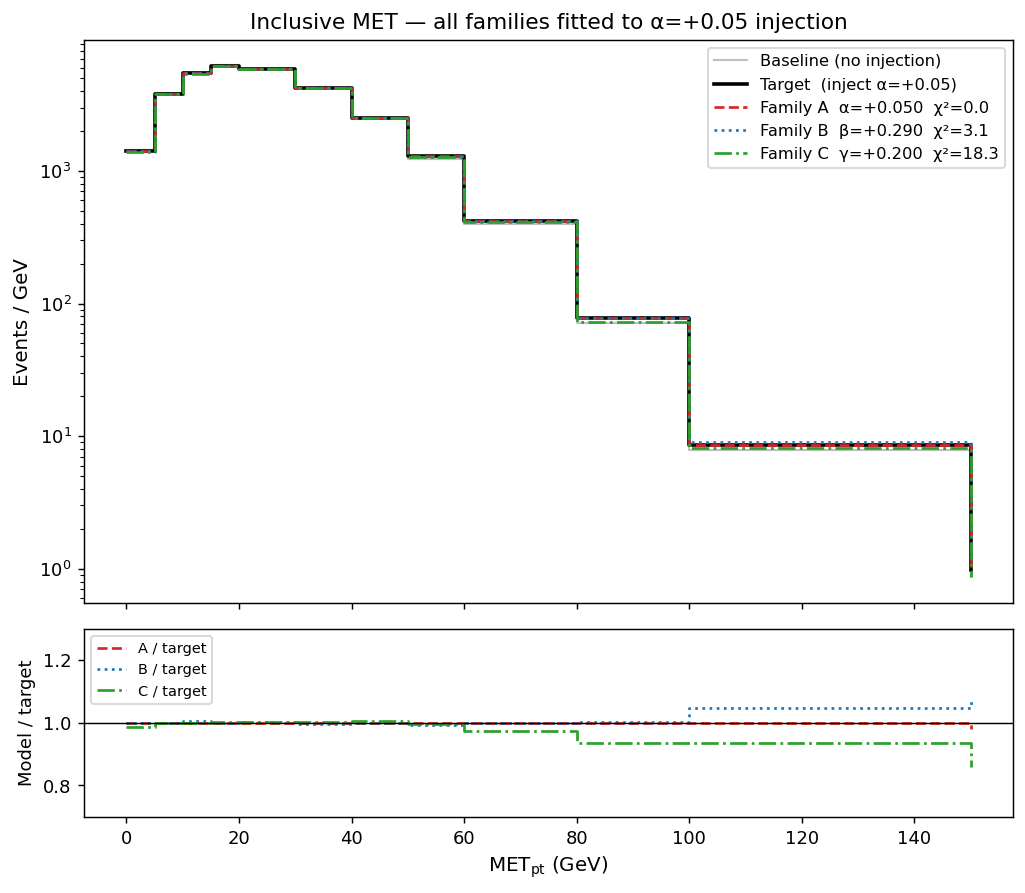
\includegraphics[width=0.85\linewidth]{met_familyA_vs_familyB.png}
  \caption{Inclusive \MET distributions for the target (black), Family~A
    (dashed red), Family~B (dotted blue), and Family~C (dash-dot green) on
    a logarithmic scale.
    The lower panel shows the ratio of each model to the target.
    Family~B achieves $\chi^2(B) = 3.13$ ($\mathrm{dof} = 11$,
    $p = 0.989$); Family~C achieves $\chi^2(C) = 18.28$
    ($\mathrm{dof} = 11$, $p = 0.075$).
    The sample comprises 233\,524 \zmumu candidates from CMS Open Data
    (DoubleMuon 2016).}
  \label{fig:inclusive}
\end{figure}

\begin{figure}[H]
  \centering
  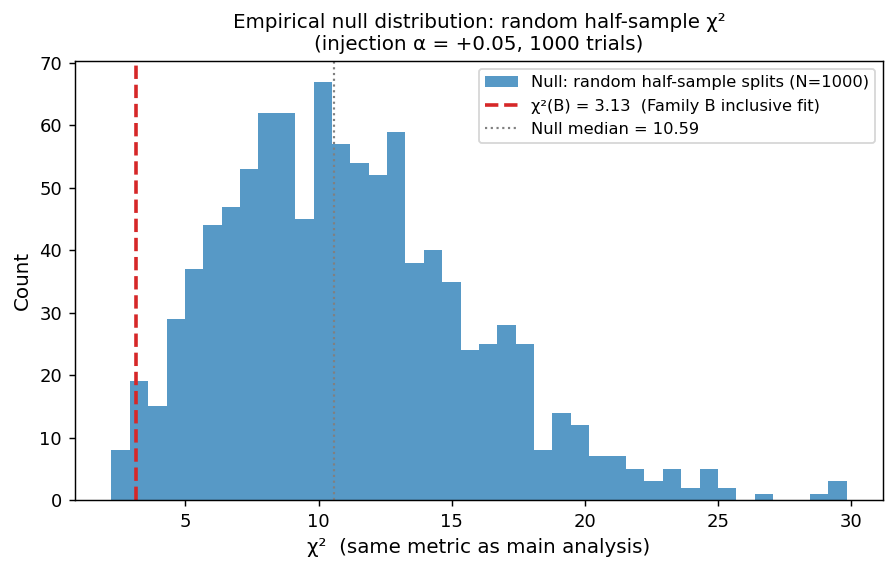
\includegraphics[width=0.75\linewidth]{null_chi2_distribution.png}
  \caption{Empirical null distribution of the inclusive \chisq statistic
    from 1\,000 bootstrap resamplings of the target \MET histogram (blue).
    Each bootstrap sample draws 233\,524 events with replacement from the
    target.
    The dashed red line marks $\chi^2(B) = 3.13$, the inclusive fit for
    Family~B.
    The null median is $\chi^2 = 10.6$ (dotted grey).
    Family~B falls at the 1.2nd percentile of the null, confirming that
    the inclusive agreement is well within the sampling noise floor of the
    target distribution.}
  \label{fig:bootstrap}
\end{figure}

\subsection{Recoil-Stratified \texorpdfstring{\MET}{MET} Distributions}

Both models were evaluated --- without refitting --- in four \pTZ strata
following the protocol binning: $[0,10)$, $[10,30)$, $[30,60)$, and
$\geq\!60\,\mathrm{GeV}$.
The separation is quantified using $\Dchisq = \chi^2(B) - \chi^2(A)$,
evaluated within each stratum while keeping the nuisance parameters fixed
at the values obtained from the inclusive fit.

\begin{table}[H]
  \centering
  \caption{Per-stratum discrimination by recoil activity.
    $\Delta\chi^2 = \chi^2(B) - \chi^2(A)$ is evaluated in each \pTZ bin
    using the best-fit parameters from the inclusive fit only.}
  \label{tab:recoil_strat}
  \begin{tabular}{lcc}
    \toprule
    \pTZ bin (GeV) & $N$ & $\Delta\chi^2$ \\
    \midrule
    $< 10$               & 92\,608 & 392 \\
    $10 \leq \pTZ < 30$  & 89\,387 &  95 \\
    $30 \leq \pTZ < 60$  & 34\,312 & 513 \\
    $\geq 60$            & 17\,217 & 1\,432 \\
    \bottomrule
  \end{tabular}
\end{table}

The overall trend is that $\Dchisq$ grows with recoil activity, with the
largest separation in the highest \pTZ bin ($\Dchisq = 1{,}432$) and the
smallest in the 10--30\,GeV bin ($\Dchisq = 95$).
This pattern is consistent with the design of Family~A, which produces \MET
distortions proportional to \pTZ.

\begin{figure}[H]
  \centering
  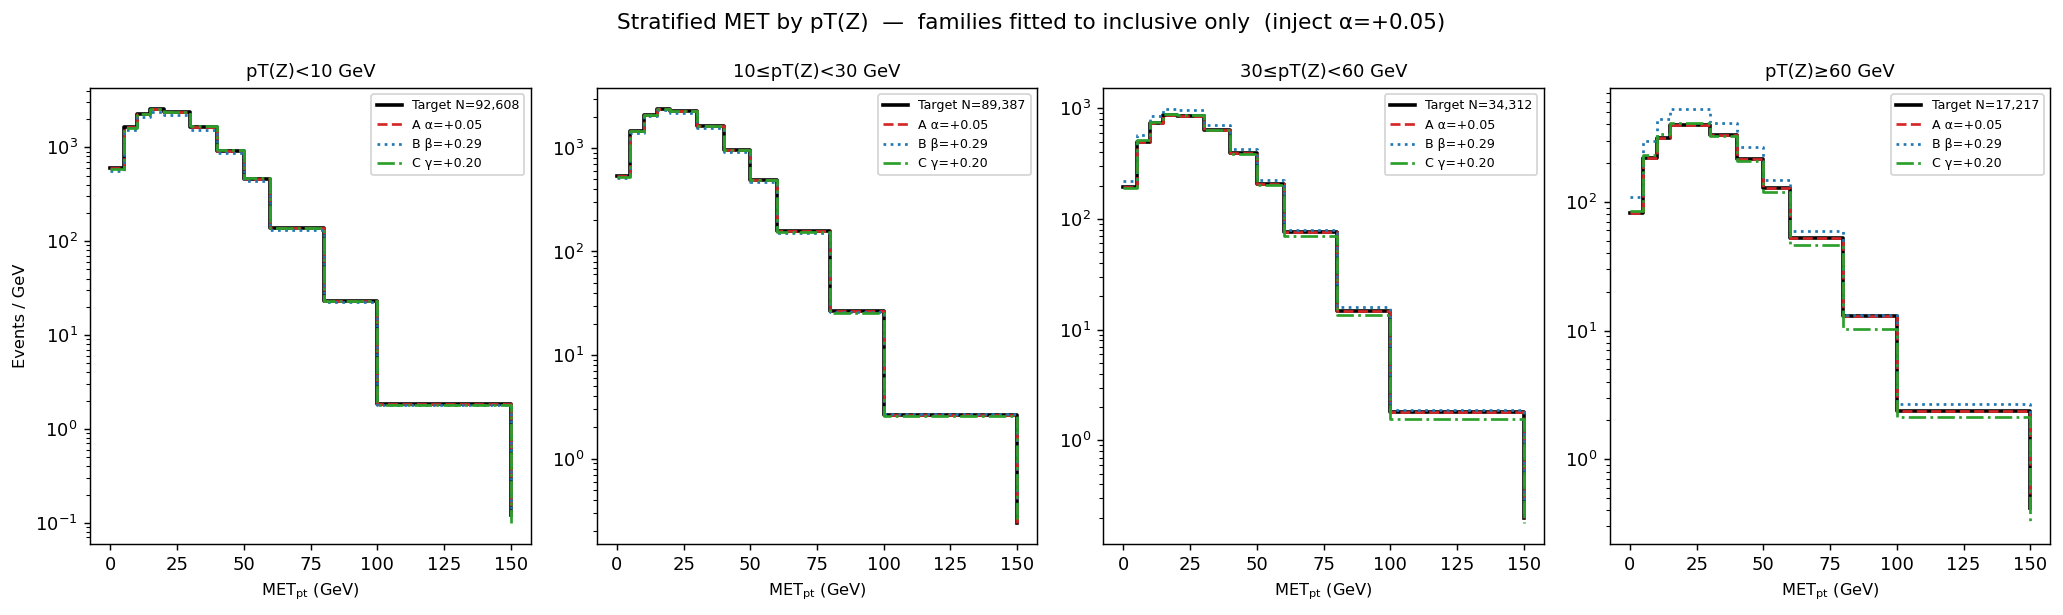
\includegraphics[width=\linewidth]{met_familyA_vs_familyB_by_zpt.png}
  \caption{\MET distributions in four \pTZ strata:
    $< 10\,\mathrm{GeV}$ ($N = 92\,608$),
    $10$--$30\,\mathrm{GeV}$ ($N = 89\,387$),
    $30$--$60\,\mathrm{GeV}$ ($N = 34\,312$), and
    $\geq\!60\,\mathrm{GeV}$ ($N = 17\,217$).
    Target (black), Family~A (dashed red), Family~B (dotted blue), and
    Family~C (dash-dot green) are shown at inclusive best-fit parameters
    without per-stratum refitting.
    The per-stratum discrimination $\Delta\chi^2(B) = \chi^2(B) -
    \chi^2(A)$ grows with recoil activity, reaching
    $\Delta\chi^2 = 1{,}432$ in the highest bin.}
  \label{fig:stratified_zpt}
\end{figure}

\subsection{Jet-Multiplicity Stratification}

Both models were evaluated after conditioning on the number of jets with
$p_{\mathrm{T}} > 30\,\mathrm{GeV}$, cleaned against the selected $Z$
muons using $\Delta R > 0.4$.

\begin{table}[H]
  \centering
  \caption{Per-stratum discrimination by jet multiplicity.
    $\Delta\chi^2 = \chi^2(B) - \chi^2(A)$ evaluated using best-fit
    parameters from the inclusive fit.}
  \label{tab:jet_strat}
  \begin{tabular}{lcc}
    \toprule
    Jet bin & $N$ & $\Delta\chi^2$ \\
    \midrule
    0-jet          & 171\,385 & 1\,405 \\
    1-jet          &  44\,706 & 1\,421 \\
    $\geq\!2$-jet  &  17\,433 & 3\,415 \\
    \bottomrule
  \end{tabular}
\end{table}

Family~B assigns global event weights of approximately 0.91, 1.17, and 1.44
to the 0-jet, 1-jet, and $\geq\!2$-jet categories respectively at
$\beta = +0.290$, producing a 44\% event-count inflation in the
$\geq\!2$-jet stratum relative to the target.
The $\geq\!2$-jet bin produces the largest per-stratum $\Dchisq$
($= 3{,}415$), reflecting this count inflation.

\begin{figure}[H]
  \centering
  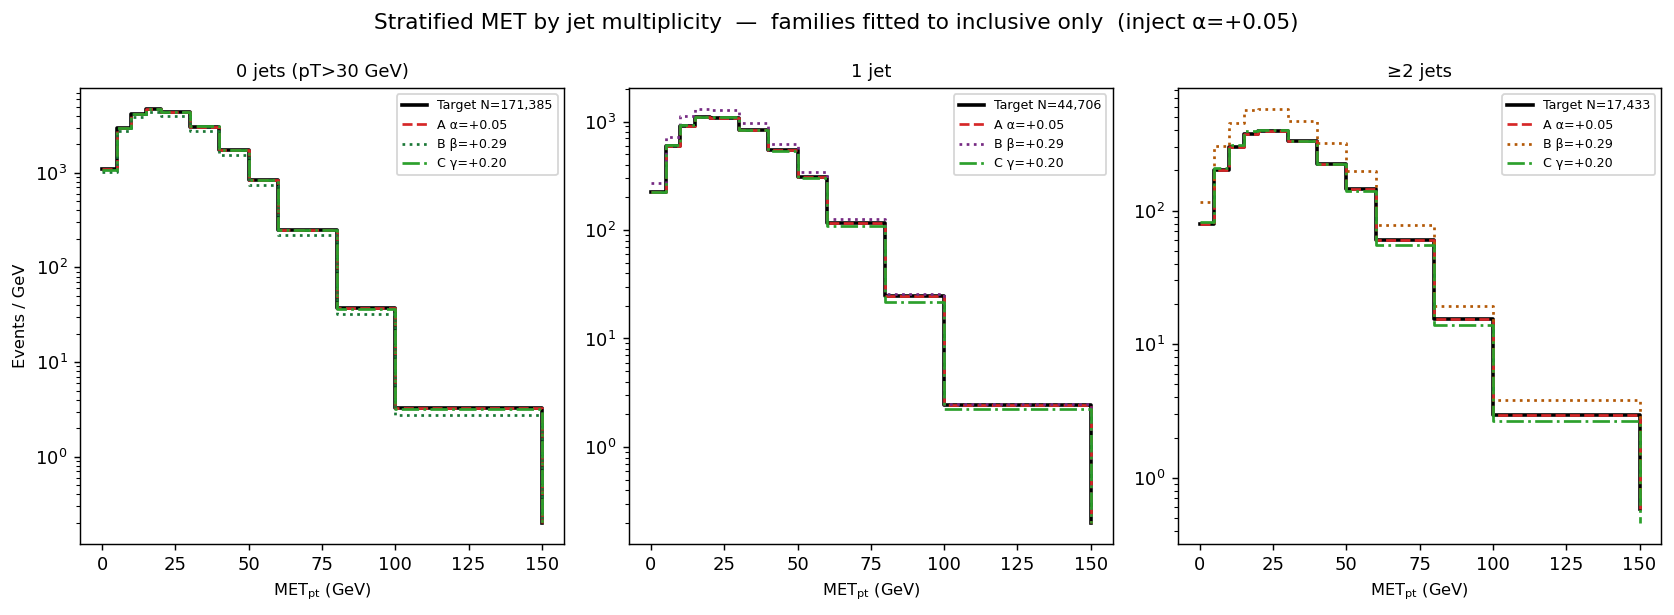
\includegraphics[width=0.90\linewidth]{met_familyA_vs_familyB_by_njets.png}
  \caption{\MET distributions stratified by jet multiplicity for
    233\,524 selected \zmumu events.
    Three categories: 0-jet ($N = 171\,385$), 1-jet ($N = 44\,706$),
    and $\geq\!2$-jet ($N = 17\,433$).
    Target (black), Family~A (dashed red), Family~B (dotted blue), and
    Family~C (dash-dot green) are evaluated at the inclusive best-fit
    parameters without refitting.
    Family~B inflates the $\geq\!2$-jet event count by approximately 44\%
    relative to the target, yielding $\Delta\chi^2(B) = 3{,}415$.
    Family~A achieves $\chi^2(A) \approx 0$ throughout.}
  \label{fig:stratified_njets}
\end{figure}

\subsection{Robustness to \texorpdfstring{\MET}{MET} Binning}

The inclusive degeneracy was evaluated under two alternative \MET binning
schemes in addition to the baseline (12 bins): a coarser binning with
9 bins, and a tail-emphasised binning with modified boundaries above
50\,GeV.
In all three cases, $\chi^2(A) = 0$ and the $p$-value for Family~B exceeded
0.96.
The inclusive degeneracy at the working point $\alpha_0 = 0.05$ persisted
under all tested binning schemes.

\subsection{Physically Grounded Public-Tier Nuisance Variation}

To test whether the inclusive degeneracy extends beyond the
phenomenological nuisance families, a third nuisance family (Family~C) is
constructed based on detector-level systematic variations exposed directly
in the CMS NanoAOD format.

NanoAOD provides event-level shifts corresponding to the CMS
unclustered-energy systematic variation through the branches
\texttt{MET\_MetUnclustEnUpDeltaX} and
\texttt{MET\_MetUnclustEnUpDeltaY}.
Family~C is defined by:
\begin{equation}
  E_{\mathrm{T},C}^{\mathrm{miss}} =
    \sqrt{\bigl(E_{\mathrm{T},x}^{\mathrm{miss}} + \gamma\,\Delta X\bigr)^2
        + \bigl(E_{\mathrm{T},y}^{\mathrm{miss}} + \gamma\,\Delta Y\bigr)^2}
  \label{eq:familyC}
\end{equation}
where $\gamma$ scales the magnitude of the systematic shift, with
$\gamma = 1$ corresponding to the full CMS unclustered-energy-up
variation.
The parameter search range is $\gamma \in [-3.0, +3.0]$ in steps of 0.05.

Fitting Family~C to the inclusive target produced by the recoil-response
injection ($\alpha = 0.05$) yields $\gamma = +0.200$, corresponding to
approximately 20\% of the full CMS unclustered-energy shift.
The resulting inclusive fit quality is $\chi^2(C) = 18.28$
($\mathrm{dof} = 11$, $p = 0.075$).

The inclusion of a nuisance perturbation derived directly from CMS
systematic-variation branches demonstrates that the observed degeneracy is
not restricted to the phenomenological toy models used for illustration,
but can arise from physically grounded detector-response variations
available in the public data representation.

Conditional projections again expose discrepancies between Family~C and the
injected recoil model.
The recoil-stratified comparison produces $\Delta\chi^2(C)$ of
$\{17, 5, 19, 58\}$ across the four \pTZ strata.
The contrast with the topology-mixture family is particularly pronounced in
the highest recoil bin: the topology-mixture model produces
$\Delta\chi^2(B) = 1{,}432$ whereas the unclustered-energy perturbation
yields $\Delta\chi^2(C) = 58$.
The jet-multiplicity stratification yields $\Delta\chi^2(C)$ of
$\{11, 26, 24\}$ for the 0-jet, 1-jet, and $\geq\!2$-jet categories
respectively.

The smaller stratified discrepancies observed for Family~C reflect a
difference in failure mode.
The unclustered-energy perturbation modifies the \MET vector while
preserving the event-topology composition of the sample.
As a result, jet-multiplicity conditioning does not directly expose a
population inconsistency, in contrast to the topology-mixture family whose
global reweighting violates the relative event counts across jet categories.

A summary of identifiability across all three nuisance families is given in
Table~\ref{tab:summary}.

\begin{table}[H]
  \centering
  \caption{Summary of identifiability across all three nuisance families
    at the working point $\alpha_0 = 0.05$.
    Inclusive $p$-value and maximum per-stratum $\Delta\chi^2$ are reported
    for each family.
    Higher inclusive $p$-value indicates deeper degeneracy with the
    injected target; higher max $\Delta\chi^2$ indicates stronger
    conditional exposure.}
  \label{tab:summary}
  \begin{tabular}{llccc}
    \toprule
    Family & Mechanism & Inclusive $\chi^2$ & $p$-value & max\,$\Delta\chi^2$ \\
    \midrule
    A & Injected truth           &  0.00 & ---   & 0 \\
    B & Topology-mixture         &  3.13 & 0.989 & 3\,415 \\
    C & Unclustered-energy shift & 18.28 & 0.075 & 58 \\
    \bottomrule
  \end{tabular}
\end{table}

The identifiability landscape (Fig.~\ref{fig:identifiability_landscape})
provides a compact visual summary of these results: Family~B occupies the
upper-right region --- deep inclusive degeneracy combined with large
conditional discrepancy --- while Family~C lies near the inclusive
acceptance boundary with modest conditional exposure.

%%===========================================================================
\section{Discussion}
\label{sec:discussion}
%%===========================================================================

\subsection{Inclusive Degeneracy and Reduced Observability}

Although the empirical example studied here involves missing transverse
momentum, the mechanism responsible for the degeneracy arises from
observable compression and therefore applies broadly to collider analyses
that rely on reduced summary observables.
As demonstrated in Section~\ref{sec:results}, the inclusive \MET
distribution admits both nuisance families despite the large event sample.
The topology-mixture model achieves $\chi^2(B) = 3.13$ on 11 degrees of
freedom ($p = 0.989$), a fit quality statistically indistinguishable from
the injected recoil-response model that generated the target distribution.

This result indicates a practical non-identifiability of nuisance
explanations in the inclusive projection: the observed data are consistent
with more than one generative model, and no hypothesis test on the inclusive
projection can select among them.
The non-identifiability here is not a consequence of insufficient data ---
233\,524 events is a large sample by typical analysis standards --- but of
insufficient observable dimensionality relative to the complexity of the
nuisance space being probed.

The explanation lies in the nature of the inclusive projection.
Both Family~A and Family~B alter the single-observable distribution
$P(\MET)$ through mechanistically different operations.
Family~A applies a continuous \MET scale factor that grows with \pTZ.
Family~B applies global per-event weights that shift the event-topology
mixture, altering the effective composition of the sample without altering
the \MET scale within any given topology.
At a sufficiently small distortion amplitude, the integrated shape changes
produced by these two mechanisms can be made to agree to within statistical
noise on the marginal distribution.

This generalises a known challenge in \MET analyses: inclusive validation
distributes sensitivity across the entire observable space, potentially
concentrating statistical power where signal-to-background from nuisance
effects is weakest.
While the empirical example studied here involves missing transverse energy,
the mechanism arises from observable compression and therefore applies to
any collider analysis relying on reduced summary observables.

\subsection{Stratified Diagnostics as Identifiability Tests}

The stratified analyses demonstrate that the non-identifiability of the
inclusive distribution does not reflect a fundamental indistinguishability
of the two nuisance models.
More precisely, the result has the structure:
$P(Y|M_1) \approx P(Y|M_2)$ yet $P(Y|Z, M_1) \neq P(Y|Z, M_2)$,
where $Y = \MET$, $M_1$ and $M_2$ denote the two nuisance families, and
$Z$ is a retained structural variable such as \pTZ or jet multiplicity.

The \pTZ stratification tests the recoil--\MET relationship.
The result is $\Dchisq$ values ranging from 95 in the 10--30\,GeV stratum
to 1\,432 in the $\geq\!60\,\mathrm{GeV}$ stratum, a discrimination of
three orders of magnitude relative to the inclusive $\chi^2(B) = 3.13$.

The jet-multiplicity stratification tests a different latent assumption:
population consistency across event topologies.
Family~B produces approximately 44\% more events in the $\geq\!2$-jet
stratum than the target, a count inflation that generates
$\Dchisq = 3{,}415$ in that bin.

The two stratifications therefore probe different latent assumptions of the
alternative model: the \pTZ test examines the recoil--\MET relationship,
while the jet-multiplicity test examines population consistency across event
topologies.
A nuisance model that passes both conditioning tests would need to jointly
preserve the recoil--\MET relationship and the jet-category population
fractions --- a substantially more constrained requirement than agreement
on the marginal \MET distribution alone.

Considering the three nuisance families together reveals that
identifiability in reduced-observability analyses is graded rather than
binary.
The topology-mixture family produces a deep inclusive degeneracy that is
strongly exposed by stratification, whereas the unclustered-energy
perturbation occupies a boundary regime in which the inclusive projection
is only marginally discriminating and conditional diagnostics produce
moderate discrepancies.

\subsection{Implications for Analyses Using Compressed Public Datasets}

Public analysis formats such as NanoAOD provide a reduced set of
reconstructed observables and omit low-level detector quantities,
effectively compressing the dimensionality of the observable event space.
This reduction has a direct implication for identifiability: as the
dimensionality of the observable space decreases, the probability that
$P(X)$ is degenerate across distinct nuisance models increases for any
single observable $X$.

The conditional projections used here represent a minimal response to this
issue, requiring only the stratification variables \pTZ and jet multiplicity
that are already present in NanoAOD.
The approach requires no additional data access and imposes no significant
computational overhead beyond the initial inclusive fit.

Within collaboration analyses, $Z\to\ell\ell$ control samples are routinely
used to constrain recoil-related nuisances in precision measurements such as
the $W$ boson mass~\cite{Kotwal:2024}; the question addressed here is how
much of that discriminating power remains available at the NanoAOD tier to
an external analyst without full systematic-variation access.

Although this study focuses on missing transverse momentum, the same
inference structure can arise for any reduced collider observable obtained
through a lossy projection of the event record --- including jet mass,
$b$-tag discriminants, and trigger-level summary observables.

\subsection{Limitations and Scope of the Demonstration}

Several limitations bound the conclusions that can be drawn from this study.
First, only two phenomenological nuisance families are compared; the
demonstration does not characterise the full space of
inclusive-indistinguishable models.
Second, the analysis is restricted to a single decay channel (\zmumu) and a
single observable (\MET).
Third, the nuisance families were constructed to be analytically tractable,
not to represent the most realistic models of detector effects.
Fourth, the inclusive degeneracy is established at a specific working point
($\alpha_0 = 0.05$, $\beta = +0.290$); the supplementary threshold sweep
shows that inclusive discrimination is restored for $\alpha_0 \geq 0.10$.

These limitations notwithstanding, the central finding is robust: inclusive
\MET in \zmumu events from CMS Open Data admits a topology-mixture
explanation at a physically plausible distortion amplitude, and two targeted
conditional projections suffice to expose the failure of that explanation.
Within these limitations, the example provides a concrete demonstration that
inclusive validation tests alone may be insufficient to guarantee
interpretability in reduced-observability collider analyses.

The degeneracies demonstrated here arise from the restricted observable
space of compressed public data tiers such as NanoAOD; they do not imply
limitations in collaboration-internal analyses, which typically exploit
higher-dimensional observables and systematic variation branches unavailable
in the public format.

%%===========================================================================
\section{Conclusions}
\label{sec:conclusions}
%%===========================================================================

A total of 233\,524 \zmumu candidate events were selected from CMS Open
Data and used to compare two physically distinct nuisance families on the
inclusive missing transverse momentum distribution.
The topology-mixture family (Family~B), fitted by grid search to the same
target as the injected recoil-response family (Family~A), achieves
$\chi^2(B) = 3.13$ on 11 degrees of freedom ($p = 0.989$).
The inclusive \MET distribution does not reject the topology-mixture
nuisance family at the working point $\alpha_0 = 0.05$, despite more than
$2 \times 10^5$ selected events.

Stratified analyses applied without refitting recover the discriminating
information absent from the inclusive projection.
Conditioning on \pTZ yields $\Dchisq = \chi^2(B) - \chi^2(A) = 1{,}432$
in the highest \pTZ bin ($\pTZ \geq 60\,\mathrm{GeV}$), with values
growing monotonically with recoil activity.
Conditioning on jet multiplicity yields $\Dchisq = 3{,}415$ in the
$\geq\!2$-jet bin, reflecting the failure of the topology-mixture model to
preserve the conditional event population across jet categories.

A supplementary test using the CMS unclustered-energy systematic variation
shows that physically grounded perturbations can also approach inclusive
degeneracy, though with weaker conditional discrepancies than the
topology-mixture family.
The comparison of three distinct nuisance families demonstrates that
reduced-tier identifiability is not an all-or-nothing property but a
spectrum determined by how the underlying mechanism projects onto the
observable space.

The general principle illustrated is that inclusive validation constrains
the marginal distribution $P(\MET)$, while stratified diagnostics probe
conditional distributions $P(\MET|S)$, where $S$ is a physics-motivated
stratification variable.
When analyses are performed on compressed data formats such as NanoAOD, the
reduced dimensionality of the observable space increases the probability
that $P(\MET)$ is degenerate across distinct nuisance models.
Conditional projections provide a minimal mechanism to restore partial
identifiability using the variables already available at the NanoAOD tier,
without requiring access to lower-level detector information.

Identifiability diagnostics of the type demonstrated here should accompany
inclusive validation tests in analyses that rely on inclusive nuisance
estimation from compressed public datasets.
The central finding --- that inclusive \MET in \zmumu events admits multiple
nuisance explanations at physically plausible distortion amplitudes, while
stratified projections distinguish them --- demonstrates the
interpretability risk in reduced-observability analyses and points toward a
straightforward mitigation strategy.
The use of real CMS Open Data events ensures that the observed degeneracy
arises from properties of reduced collider observables themselves rather
than artefacts of a particular simulation framework.
The analysis therefore illustrates a general limitation of inference based
on reduced collider observables: agreement in inclusive validation
distributions does not guarantee that the underlying nuisance mechanisms are
uniquely determined.
More broadly, the example illustrates how compression of collider events
into reduced analysis tiers can alter the structure of statistical
inference, introducing nuisance degeneracies that are invisible to inclusive
validation but recoverable through conditional diagnostics.

%%===========================================================================
\section*{Data Availability}
%%===========================================================================

The CMS Open Data used in this analysis are publicly available through the
CERN Open Data Portal (\url{https://opendata.cern.ch}).
The specific dataset is the CMS 2016 DoubleMuon NanoAOD, accessible at
the URL documented in Ref.~\cite{CMSOpenData:2016}.
All analysis scripts, the frozen protocol document, and SHA-256 checksums
for input data files are available in the accompanying repository at
\url{https://github.com/blumhardt-m/zmet-nid}, tagged at the version
corresponding to this submission.
NanoAOD files were accessed and processed using
uproot~\cite{Pivarski:uproot} and Awkward Array~\cite{Pivarski:2018}
from the Scikit-HEP ecosystem~\cite{Rodrigues:2020}.

%%===========================================================================
\section*{AI Assistance Disclosure}
%%===========================================================================

Portions of the analysis code and manuscript text were developed with
assistance from Claude (Anthropic) and Claude Code.
All scientific decisions, experimental design, protocol definitions, and
conclusions are the sole responsibility of the author.
AI-assisted code was reviewed, tested, and validated by the author prior to
use.
The frozen protocol governing this analysis predates and is independent of
any AI-assisted implementation steps.

%%===========================================================================
\begin{thebibliography}{99}
%%===========================================================================

\bibitem{CMSOpenData:2016}
  CERN Open Data Portal,
  \emph{CMS Open Data --- DoubleMuon Run2016B, RunIISummer16NanoAODv7},
  \url{https://opendata.cern.ch} (accessed 2026).

\bibitem{CMSOpenDataGuide}
  CMS Collaboration,
  \emph{CMS Open Data Guide},
  \url{https://cms-opendata-guide.web.cern.ch} (accessed 2026).

\bibitem{CMS:MiniNanoAOD}
  CMS Collaboration,
  \emph{The CMS MiniAOD and NanoAOD data formats},
  CMS Physics Analysis Summary CMS-PAS-GEN-19-002 (2019).

\bibitem{Rizzi:2019}
  A.~Rizzi, G.~Petrucciani and M.~Peruzzi,
  on behalf of the CMS Collaboration,
  \emph{A further reduction in CMS event data for analysis: the NANOAOD
    format},
  \emph{EPJ Web Conf.}~\textbf{214} (2019) 06021
  [\href{https://doi.org/10.1051/epjconf/201921406021}{doi:10.1051/epjconf/201921406021}].

\bibitem{CMS:MET2019}
  CMS Collaboration,
  \emph{Performance of missing transverse momentum reconstruction in
    proton-proton collisions at $\sqrt{s} = 13\,\mathrm{TeV}$ using the
    CMS detector},
  \emph{JINST}~\textbf{14} (2019) P07004
  [\href{https://doi.org/10.1088/1748-0221/14/07/P07004}{doi:10.1088/1748-0221/14/07/P07004}].

\bibitem{CMS:JES2017}
  CMS Collaboration,
  \emph{Jet energy scale and resolution in the CMS experiment in pp
    collisions at 8\,TeV},
  \emph{JINST}~\textbf{12} (2017) P02014
  [\href{https://doi.org/10.1088/1748-0221/12/02/P02014}{doi:10.1088/1748-0221/12/02/P02014}].

\bibitem{CMS:Muon2018}
  CMS Collaboration,
  \emph{Performance of the CMS muon detector and muon reconstruction with
    proton-proton collisions at $\sqrt{s} = 13\,\mathrm{TeV}$},
  \emph{JINST}~\textbf{13} (2018) P06015
  [\href{https://doi.org/10.1088/1748-0221/13/06/P06015}{doi:10.1088/1748-0221/13/06/P06015}].

\bibitem{PDG:2020}
  Particle Data Group, P.A.~Zyla et al.,
  \emph{Review of Particle Physics},
  \emph{Prog. Theor. Exp. Phys.}~\textbf{2020} (2020) 083C01
  [\href{https://doi.org/10.1093/ptep/ptaa104}{doi:10.1093/ptep/ptaa104}].

\bibitem{Pivarski:2018}
  J.~Pivarski et al.,
  \emph{Awkward Array},
  Zenodo (2018--present)
  [\href{https://doi.org/10.5281/zenodo.4341376}{doi:10.5281/zenodo.4341376}].

\bibitem{Pivarski:uproot}
  J.~Pivarski, P.~Nandi et al.,
  \emph{uproot},
  Zenodo (2017--present)
  [\href{https://doi.org/10.5281/zenodo.4340632}{doi:10.5281/zenodo.4340632}].

\bibitem{Rodrigues:2020}
  E.~Rodrigues et al.,
  \emph{The Scikit-HEP project},
  \emph{EPJ Web Conf.}~\textbf{245} (2020) 06028
  [\href{https://doi.org/10.1051/epjconf/202024506028}{doi:10.1051/epjconf/202024506028}].

\bibitem{Cranmer:2014}
  K.~Cranmer,
  \emph{Practical Statistics for the LHC},
  CERN Yellow Report CERN-2014-003 (2014)
  [\href{https://arxiv.org/abs/1503.07622}{arXiv:1503.07622}].

\bibitem{Valsecchi:2026}
  D.~Valsecchi, M.~Doneg{\`a} and R.~Wallny,
  \emph{Profiling systematic uncertainties in Simulation-Based Inference
    with Factorizable Normalizing Flows},
  arXiv:2602.13184 (2026).

\bibitem{ATLAS:2024}
  ATLAS Collaboration,
  \emph{An implementation of neural simulation-based inference for
    parameter estimation in ATLAS},
  arXiv:2412.01600 (2024).

\bibitem{Kotwal:2024}
  A.V.~Kotwal,
  \emph{The precision measurement of the $W$ boson mass and its impact on
    physics},
  arXiv:2409.08244 (2024).

\end{thebibliography}

\end{document}
